\documentclass[11pt,a4paper]{article}
\usepackage[T1]{fontenc}
\usepackage[utf8]{inputenc}
\usepackage{lmodern}
\usepackage[margin=2.3cm]{geometry}
\usepackage{microtype}
\usepackage{booktabs}
\usepackage{array}
\usepackage{xcolor}
\usepackage{tikz}
\usetikzlibrary{arrows.meta,positioning,shapes.geometric,calc,fit,backgrounds,decorations.pathreplacing,patterns}
\usepackage{pgfplots}
\pgfplotsset{compat=1.17}
\usepackage{enumitem}
\usepackage{caption}
\usepackage[hidelinks]{hyperref}

\definecolor{ink}{HTML}{1B2430}
\definecolor{ink2}{HTML}{525C68}
\definecolor{mute}{HTML}{8A939E}
\definecolor{copper}{HTML}{B5551D}
\definecolor{iso}{HTML}{3B6EA8}
\definecolor{good}{HTML}{2E7D5B}
\definecolor{warn}{HTML}{C98A1B}
\definecolor{crit}{HTML}{B3372F}
\definecolor{panel}{HTML}{EEF0EB}
\definecolor{line}{HTML}{D9DDD6}

\setlist{nosep,leftmargin=1.4em}
\captionsetup{font=small,labelfont=bf,labelsep=period}
\setlength{\parskip}{4pt}
\setlength{\parindent}{0pt}

\tikzset{
  box/.style={draw=ink2,fill=white,rounded corners=2pt,align=center,font=\small,inner sep=5pt,minimum height=9mm},
  pubbox/.style={box,draw=iso,fill=iso!8},
  privbox/.style={box,draw=crit,fill=crit!8},
  modbox/.style={box,draw=copper,fill=copper!10},
  lab/.style={font=\footnotesize\color{ink2}},
  arr/.style={-{Latex[length=2mm]},draw=ink2,thick},
}

\title{\vspace{-1.2cm}\textbf{Two experiments on public grid data}\\[4pt]
\large Predicting interconnection constraints and network-upgrade slippage from what the public can see}
\author{Luke Blommesteyn}
\date{September 2026}

\begin{document}
\maketitle
\vspace{-0.8cm}

\begin{center}
\begin{minipage}{0.92\textwidth}
\small\color{ink2}
Two research prototypes, built end to end and benchmarked chronologically. The first asks whether public
pre-study information can predict which transmission facilities an interconnection request will be found to
constrain. The second asks whether the public record of an ISO's own project tables can predict which
network upgrades will slip by more than a year or grow in cost by more than a quarter. Both were run
honestly, with point-in-time discipline, and both came back mostly negative. This note lays out what was
built, what the numbers say, and where the public data runs out. I would value any reaction from people who
work with this data day to day.
\end{minipage}
\end{center}

\section*{Experiment 1 --- Which facilities will a proposed project constrain?}

\textbf{Question.} Given a generator, battery or large load entering an ISO queue, using only information
public before the ISO's system impact study is published (queue history, earlier studies, nodal congestion,
outages, approximate topology), rank the transmission facilities the study will find constrained.

\textbf{Two tracks.} Real PJM study PDFs were unreachable from the build sandbox, so the method was first
developed on a \emph{simulated ISO} sitting on a real public PJM-footprint nodal case (ICARUS testbed:
17{,}467 buses, 21{,}554 branches with impedances and ratings). The simulator runs a PJM-style DC-power-flow
study procedure (DFAX, LODF contingency screening, Manual~14B-style attribution) for 2{,}640 queue requests
over 2011--2025, renders the findings as PDFs with realistic naming noise, and publishes market, outage and
upgrade data derived from the same hidden case. Models only ever see the public side. Later, the frozen
model was run unchanged on 213 real PJM impact studies fetched by a GitHub Actions runner.

\begin{figure}[h]
\centering
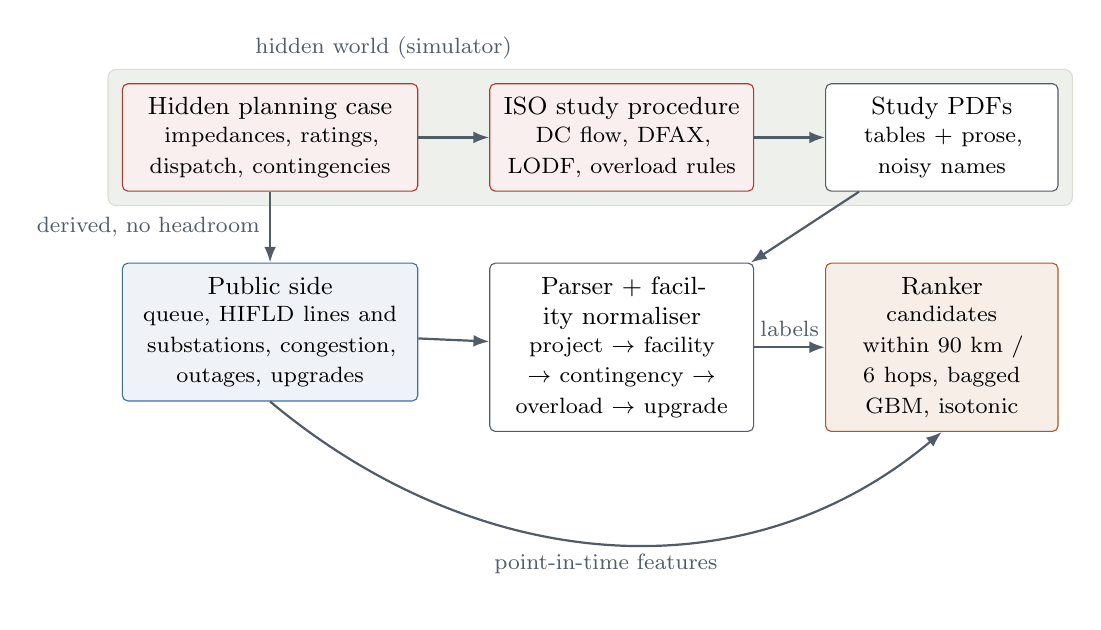
\begin{tikzpicture}[node distance=6mm and 9mm]
  \node[privbox,text width=34mm] (case) {Hidden planning case\\[-1pt]{\footnotesize impedances, ratings, dispatch, contingencies}};
  \node[privbox,text width=30mm,right=of case] (study) {ISO study procedure\\[-1pt]{\footnotesize DC flow, DFAX, LODF, overload rules}};
  \node[box,text width=26mm,right=of study] (pdf) {Study PDFs\\[-1pt]{\footnotesize tables + prose, noisy names}};
  \node[pubbox,text width=34mm,below=9mm of case] (pub) {Public side\\[-1pt]{\footnotesize queue, HIFLD lines and substations, congestion, outages, upgrades}};
  \node[box,text width=30mm,below=9mm of study] (parse) {Parser + facility normaliser\\[-1pt]{\footnotesize project $\to$ facility $\to$ contingency $\to$ overload $\to$ upgrade}};
  \node[modbox,text width=26mm,below=9mm of pdf] (model) {Ranker\\[-1pt]{\footnotesize candidates within 90 km / 6 hops, bagged GBM, isotonic}};
  \draw[arr] (case) -- (study);
  \draw[arr] (study) -- (pdf);
  \draw[arr] (pdf) -- (parse);
  \draw[arr] (case) -- node[lab,left]{derived, no headroom} (pub);
  \draw[arr] (pub) -- (parse);
  \draw[arr] (parse) -- node[lab,above]{labels} (model);
  \draw[arr] (pub.south) to[out=-40,in=-140] node[lab,below]{point-in-time features} (model.south);
  \begin{scope}[on background layer]
    \node[fit=(case)(study)(pdf),draw=line,fill=panel,rounded corners=3pt,inner sep=5pt,label={[lab]above left:hidden world (simulator)}] {};
  \end{scope}
\end{tikzpicture}
\caption{Experiment 1 layout. Everything above the line is hidden from the models; the public side is derived from the same case but carries no facility headroom (ratings, dispatch, contingency definitions).}
\end{figure}

\textbf{Point-in-time discipline.} Every feature is built from tables truncated at the observation date, and a
vintage test rebuilds the features from a table cut at that date and asserts equality. That test caught one
real leak during development (generator features computed from the full plant list).

\subsection*{Results on the simulated ISO (279 held-out projects queued after mid-2022)}

\begin{figure}[h]
\centering
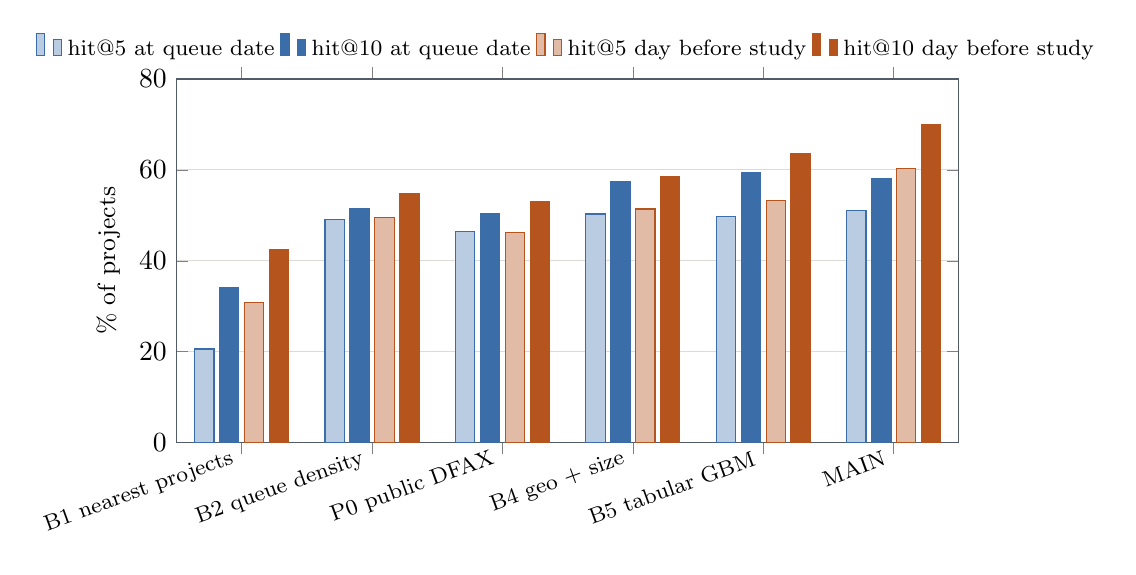
\begin{tikzpicture}
\begin{axis}[
  ybar, bar width=7pt, width=0.95\textwidth, height=6.2cm,
  ymin=0, ymax=80, ylabel={\% of projects}, ylabel style={font=\small},
  symbolic x coords={B1 nearest projects, B2 queue density, P0 public DFAX, B4 geo + size, B5 tabular GBM, MAIN},
  xtick=data, x tick label style={font=\footnotesize, rotate=20, anchor=east},
  ymajorgrids, grid style={line}, axis line style={ink2},
  legend style={font=\footnotesize, at={(0.5,1.02)}, anchor=south, draw=none, fill=none, legend columns=4},
]
\addplot[fill=iso!35, draw=iso] coordinates {(B1 nearest projects,20.6) (B2 queue density,49.0) (P0 public DFAX,46.5) (B4 geo + size,50.3) (B5 tabular GBM,49.7) (MAIN,51.0)};
\addplot[fill=iso, draw=iso] coordinates {(B1 nearest projects,34.2) (B2 queue density,51.6) (P0 public DFAX,50.3) (B4 geo + size,57.4) (B5 tabular GBM,59.4) (MAIN,58.1)};
\addplot[fill=copper!40, draw=copper] coordinates {(B1 nearest projects,30.8) (B2 queue density,49.5) (P0 public DFAX,46.3) (B4 geo + size,51.4) (B5 tabular GBM,53.2) (MAIN,60.4)};
\addplot[fill=copper, draw=copper] coordinates {(B1 nearest projects,42.4) (B2 queue density,54.9) (P0 public DFAX,53.0) (B4 geo + size,58.6) (B5 tabular GBM,63.7) (MAIN,69.9)};
\legend{hit@5 at queue date, hit@10 at queue date, hit@5 day before study, hit@10 day before study}
\end{axis}
\end{tikzpicture}
\caption{Hit@K: share of held-out projects whose actual constrained facility appears in the top K. Blue: features as of the queue date. Copper: features as of the day before the study was published (10--26 months later, 698 test projects).}
\end{figure}

\begin{itemize}
\item \textbf{Headline, queue date:} the learned model (all public feature families, bagged GBM) puts the true facility in
  the top 5 for 51.0\% of projects and the top 10 for 58.1\%. The best simple baseline, a logistic model on geography and
  size, gets 50.3\% / 57.4\%. On the headline metric the method does not materially beat geography.
\item \textbf{Where it does help:} on facilities \emph{not directly connected} to the point of interconnection, hit@5 is
  44.9\% against 40.8\%; probabilistic skill roughly doubles (Brier skill 0.095 vs 0.048); the predicted number of
  constrained facilities tracks the actual number much better (correlation 0.41 vs 0.21).
\item \textbf{Fresher information changes the picture:} evaluated with everything public up to the day before the study,
  the model reaches 60.4\% / 69.9\% against 53.2\% / 63.7\% for the best baseline. Public evidence about a facility's
  headroom (recent studies, queue movements, binding hours) decays fast in this world.
\item \textbf{What private data is missing:} handing the model the hidden case's exact impedances (true distribution
  factors) lifts hit@5 only from 51.6\% to 54.2\%. Topology is not the bottleneck; facility headroom is, and no public
  feed carries it. In a second simulated world where headroom persists between studies instead of being re-hardened
  yearly, the model's edge widens (hit@10 66.7\% vs 59.2\%).
\end{itemize}

\begin{figure}[h]
\centering
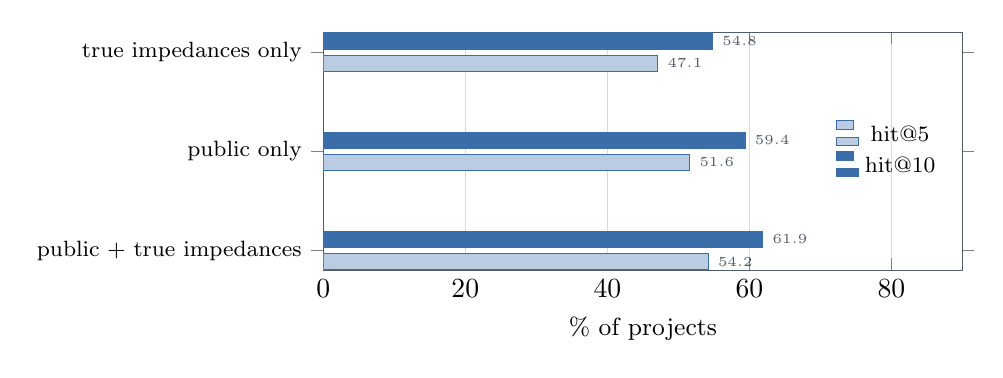
\begin{tikzpicture}
\begin{axis}[
  xbar, bar width=6pt, width=0.8\textwidth, height=4.6cm,
  xmin=0, xmax=90, xlabel={\% of projects}, xlabel style={font=\small},
  symbolic y coords={true impedances only, public only, public + true impedances},
  ytick=data, y tick label style={font=\footnotesize}, y dir=reverse,
  xmajorgrids, grid style={line}, axis line style={ink2},
  legend style={font=\footnotesize, at={(0.98,0.5)}, anchor=east, draw=none, fill=none},
  nodes near coords, every node near coord/.append style={font=\tiny, color=ink2},
]
\addplot[fill=iso!35, draw=iso] coordinates {(47.1,true impedances only) (51.6,public only) (54.2,public + true impedances)};
\addplot[fill=iso, draw=iso] coordinates {(54.8,true impedances only) (59.4,public only) (61.9,public + true impedances)};
\legend{hit@5, hit@10}
\end{axis}
\end{tikzpicture}
\caption{Oracle ablation. Giving the model the hidden impedances buys a few points; the remaining gap is headroom.}
\end{figure}

\subsection*{The frozen model on 213 real PJM impact studies}

The Actions runner fetched PJM's queue export (9{,}263 rows) and 213 impact-study PDFs for 2016--2020 requests, each
with its HTTP Last-Modified date as the publication proxy. The frozen model was scored on every study with a locatable
point of interconnection, features as of queue date plus one day, and the first benchmark was recorded before any
change was made.

\begin{center}
\small
\begin{tabular}{lrrrrr}
\toprule
& evaluable projects & hit@5 & hit@10 & recall@10 & MRR \\
\midrule
frozen model & 7 of 212 scored & 14.3\% & 42.9\% & 33.3\% & 0.12 \\
nearest-projects heuristic & 7 & 14.3\% & 57.1\% & 47.6\% & 0.10 \\
queue-density heuristic & 7 & 14.3\% & 28.6\% & 21.4\% & 0.07 \\
\bottomrule
\end{tabular}
\end{center}

With seven evaluable projects none of these differences means anything. The binding constraint is identity, not
modelling: real reports name facilities by PSS/E bus names (``8CHCKAHM--8ELMONT 500~kV''), and only 45 of 214 parsed
findings could be tied to a public HIFLD/OSM substation pair, because most substations in the public geometry carry no
name. The next real-data step is a bus-name dictionary, not a better ranker.

\vspace{4pt}
\section*{Experiment 2 --- Which network upgrades will slip or overrun?}

\textbf{Question.} For an upgrade as PJM listed it on a given day, using only what was public that day: the probability
it goes into service more than 12 months after the date PJM was publishing, the probability its estimate ends up more
than 25\% above the estimate published then, and completion-date and final-cost ranges.

\textbf{Reconstructing a table the ISO only serves once.} PJM publishes a single current version of its Project Status \&
Cost Allocation table. The longitudinal table (upgrade $\times$ observation date) was rebuilt from Internet Archive
captures of the legacy construction-status page, whose rows turned out to be embedded in ASP.NET ViewState or an inline
JSON block; from the XML data files behind the older ActiveX version of the page; and from a live export of the current
grid. This is real data throughout.

\begin{figure}[h]
\centering
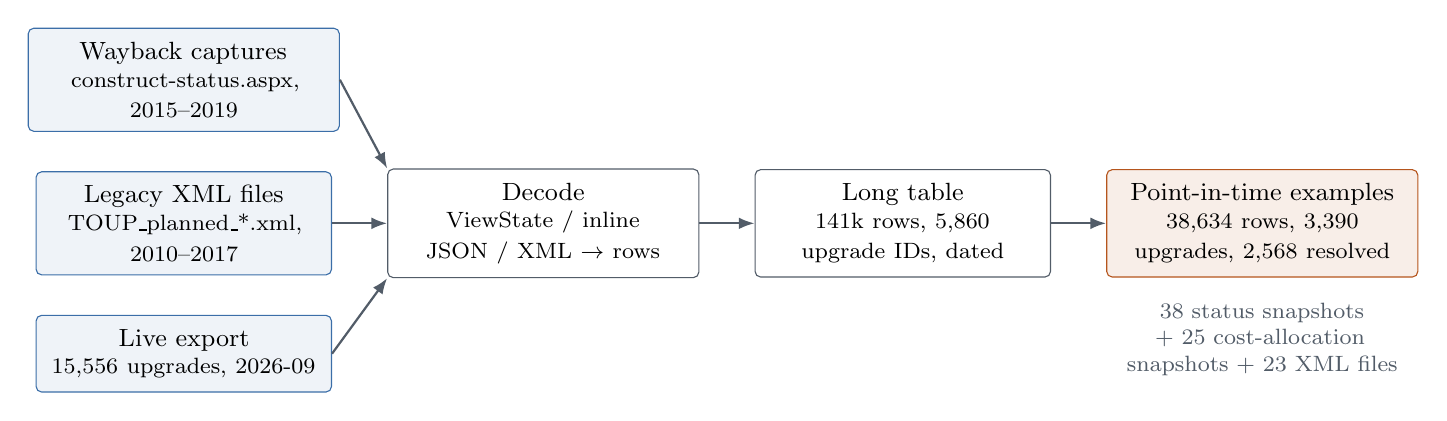
\begin{tikzpicture}[node distance=5mm and 7mm]
  \node[pubbox,text width=36mm] (wb) {Wayback captures\\[-1pt]{\footnotesize construct-status.aspx, 2015--2019}};
  \node[pubbox,text width=34mm,below=of wb] (xml) {Legacy XML files\\[-1pt]{\footnotesize TOUP\_planned\_*.xml, 2010--2017}};
  \node[pubbox,text width=34mm,below=of xml] (live) {Live export\\[-1pt]{\footnotesize 15{,}556 upgrades, 2026-09}};
  \node[box,text width=36mm,right=of xml] (dec) {Decode\\[-1pt]{\footnotesize ViewState / inline JSON / XML $\to$ rows}};
  \node[box,text width=34mm,right=of dec] (long) {Long table\\[-1pt]{\footnotesize 141k rows, 5{,}860 upgrade IDs, dated}};
  \node[modbox,text width=36mm,right=of long] (ex) {Point-in-time examples\\[-1pt]{\footnotesize 38{,}634 rows, 3{,}390 upgrades, 2{,}568 resolved}};
  \draw[arr] (wb.east) -- (dec.north west);
  \draw[arr] (xml) -- (dec);
  \draw[arr] (live.east) -- (dec.south west);
  \draw[arr] (dec) -- (long);
  \draw[arr] (long) -- (ex);
  \node[lab,below=2mm of ex,text width=36mm,align=center] {38 status snapshots + 25 cost-allocation snapshots + 23 XML files};
\end{tikzpicture}
\caption{Experiment 2 data path. The fetch runs on a GitHub Actions runner because the build sandbox cannot reach pjm.com or archive.org.}
\end{figure}

\begin{figure}[h]
\centering
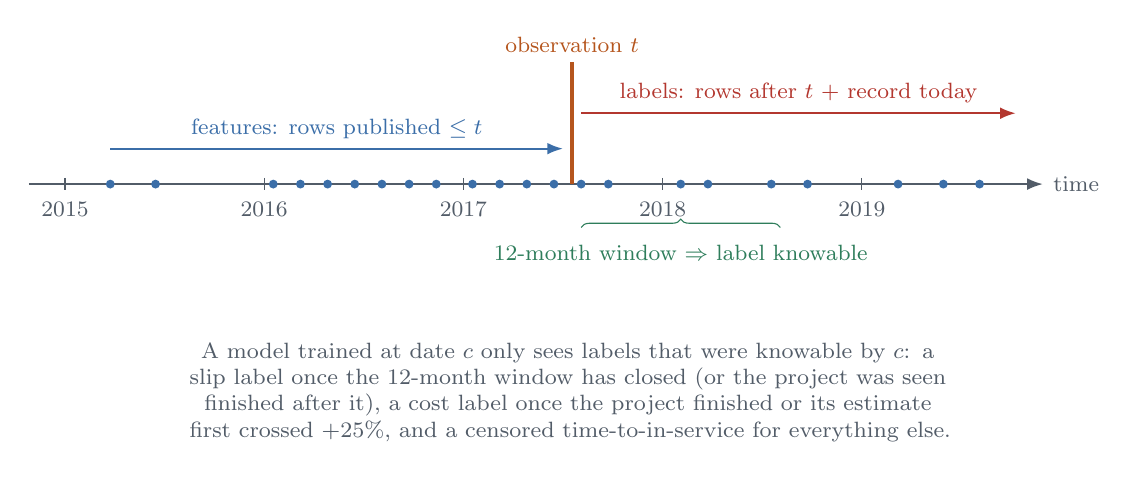
\begin{tikzpicture}[x=1.15cm]
  \draw[thick,ink2,-{Latex[length=2mm]}] (0,0) -- (11.2,0) node[right,lab]{time};
  \foreach \x/\l in {0.4/2015, 2.6/2016, 4.8/2017, 7.0/2018, 9.2/2019} {\draw[ink2] (\x,0.08) -- (\x,-0.08); \node[lab,below] at (\x,-0.1) {\l};}
  \foreach \x in {0.9,1.4,2.7,3.0,3.3,3.6,3.9,4.2,4.5,4.9,5.2,5.5,5.8,6.1,6.4,7.2,7.5,8.2,8.6,9.6,10.1,10.5} {\fill[iso] (\x,0) circle (1.6pt);}
  \draw[copper,very thick] (6.0,0) -- (6.0,1.55);
  \node[lab,copper,above] at (6.0,1.55) {observation $t$};
  \draw[arr,iso] (0.9,0.45) -- node[lab,above]{features: rows published $\le t$} (5.9,0.45);
  \draw[arr,crit] (6.1,0.9) -- node[lab,above]{labels: rows after $t$ + record today} (10.9,0.9);
  \draw[decorate,decoration={brace,amplitude=3pt},good] (6.1,-0.55) -- (8.3,-0.55) node[midway,below=3pt,lab,good]{12-month window $\Rightarrow$ label knowable};
  \node[lab,below=8mm of current bounding box.south,text width=0.9\textwidth,align=center] {A model trained at date $c$ only sees labels that were knowable by $c$: a slip label once the 12-month window has closed (or the project was seen finished after it), a cost label once the project finished or its estimate first crossed $+25\%$, and a censored time-to-in-service for everything else.};
\end{tikzpicture}
\caption{Point-in-time rules. Blue dots are archived snapshot dates. The vintage tests rebuild the features from a truncated table and assert equality, and assert that every completion-known date lies after the observation.}
\end{figure}

\textbf{Outcomes.} \emph{delay\_12m}: PJM's recorded in-service date more than 12 months after the date published at $t$
(also 1 if still unbuilt 12 months after it; cancelled projects carry no slip label). \emph{cost\_overrun\_25}: final cost
more than 25\% above the estimate at $t$ (cancelled and zero-cost records excluded). \emph{cancelled}: a separate outcome.
Slip base rate 19\%, overrun base rate 17\%, 17\% of examples censored.

\subsection*{Protocol, and the number that was not real}

The evaluation is rolling-origin: seven test months from January 2018 to December 2019; at each, every baseline and
model is refitted on all earlier observations using only labels knowable then, and scores that month. Predictions are
pooled. A first pass used a single fixed cutoff with labels taken from the full record and scored a slip AUROC of
0.835. Restricting the training labels to what was knowable dropped it to 0.58: the model had been recognising an
upgrade it had seen in training and recalling its eventual fate. Everything below uses the honest protocol.

\begin{figure}[h]
\centering
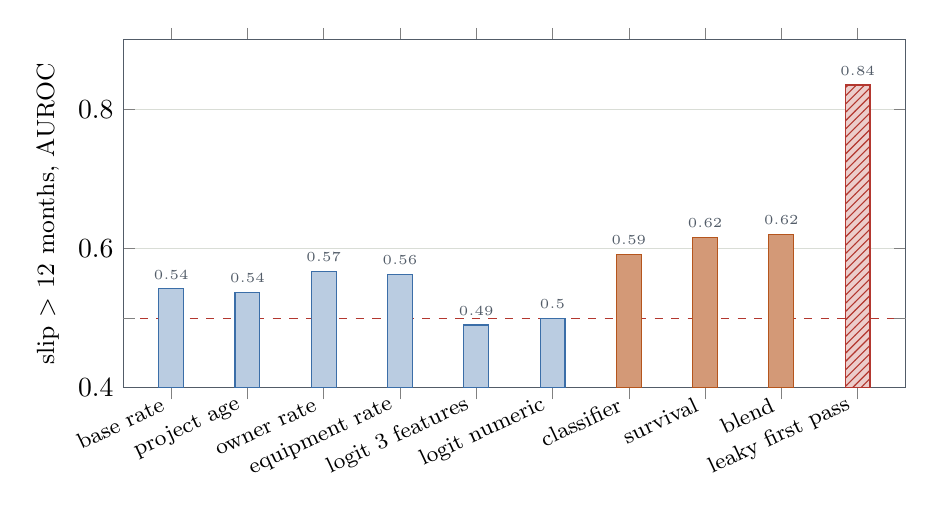
\begin{tikzpicture}
\begin{axis}[
  ybar, bar width=9pt, width=0.95\textwidth, height=6cm,
  ymin=0.4, ymax=0.9, ylabel={slip $>$ 12 months, AUROC}, ylabel style={font=\small},
  symbolic x coords={base rate, project age, owner rate, equipment rate, logit 3 features, logit numeric, classifier, survival, blend, leaky first pass},
  xtick={base rate, project age, owner rate, equipment rate, logit 3 features, logit numeric, classifier, survival, blend, leaky first pass},
  x tick label style={font=\footnotesize, rotate=25, anchor=east}, bar shift=0pt, enlarge x limits=0.07,
  ymajorgrids, grid style={line}, axis line style={ink2},
  nodes near coords, every node near coord/.append style={font=\tiny, color=ink2, /pgf/number format/fixed, /pgf/number format/precision=2},
  extra y ticks={0.5}, extra y tick labels={}, extra y tick style={grid=major, grid style={crit, dashed}},
]
\addplot[fill=iso!35, draw=iso] coordinates {(base rate,0.542) (project age,0.537) (owner rate,0.567) (equipment rate,0.563) (logit 3 features,0.490) (logit numeric,0.499)};
\addplot[fill=copper!60, draw=copper] coordinates {(classifier,0.592) (survival,0.616) (blend,0.620)};
\addplot[fill=crit!25, draw=crit, postaction={pattern=north east lines, pattern color=crit}] coordinates {(leaky first pass,0.835)};
\end{axis}
\end{tikzpicture}
\caption{Slip AUROC on the pooled 2018--2019 holdout (6{,}877 examples, 943 upgrades). Blue: baselines. Copper: the honest models. Hatched: the leaky single-cutoff pass, shown only because it is what a careless benchmark would report.}
\end{figure}

\begin{center}
\footnotesize
\begin{tabular}{lrrrrrrr}
\toprule
& \multicolumn{3}{c}{slip $>$ 12 mo} & \multicolumn{2}{c}{cost $+25\%$} & \multicolumn{2}{c}{completion month} \\
\cmidrule(lr){2-4}\cmidrule(lr){5-6}\cmidrule(lr){7-8}
model & AUROC & Brier & ECE & AUROC & Brier & P50 MAE & P90 cover \\
\midrule
always on time (PJM's own date, cost) & 0.500 & 0.201 & 0.189 & 0.500 & 0.211 & \textbf{9.3} & -- \\
base rate & 0.542 & 0.187 & 0.149 & 0.493 & \textbf{0.175} & 9.3 & 0.76 \\
owner rate (point-in-time) & 0.567 & 0.185 & 0.144 & 0.574 & 0.172 & 9.6 & 0.75 \\
logistic: voltage, cost, horizon & 0.490 & 0.198 & 0.179 & \textbf{0.621} & 0.176 & 11.1 & 0.62 \\
calibrated GBM classifier & 0.592 & 0.196 & 0.177 & 0.611 & 0.190 & 13.9 & 0.53 \\
discrete-time survival & 0.616 & 0.213 & 0.177 & -- & -- & 10.6 & 0.78 \\
blend (survival + classifier) & \textbf{0.620} & \textbf{0.172} & \textbf{0.103} & 0.611 & 0.190 & 10.6 & 0.78 \\
\bottomrule
\end{tabular}
\end{center}

\begin{figure}[h]
\centering
\begin{minipage}[t]{0.48\textwidth}\centering
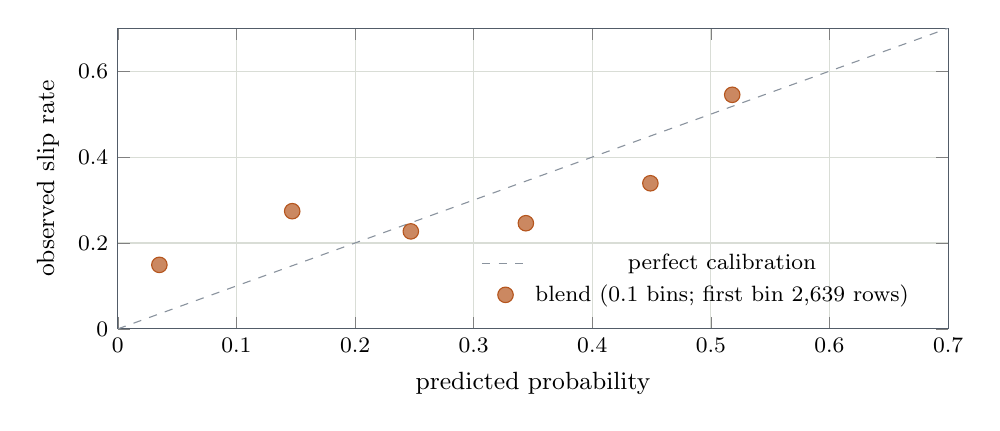
\begin{tikzpicture}
\begin{axis}[
  width=\textwidth, height=5.4cm, xmin=0, xmax=0.7, ymin=0, ymax=0.7,
  xlabel={predicted probability}, ylabel={observed slip rate}, label style={font=\small}, tick label style={font=\footnotesize},
  grid=major, grid style={line}, axis line style={ink2},
  legend style={font=\footnotesize, at={(0.97,0.04)}, anchor=south east, draw=none, fill=none},
]
\addplot[mute, dashed, domain=0:0.7] {x};
\addplot[only marks, mark=*, copper, mark options={scale=1.4, fill=copper!70}] coordinates {(0.035,0.149) (0.147,0.274) (0.247,0.227) (0.344,0.246) (0.449,0.339) (0.518,0.545)};
\legend{perfect calibration, blend (0.1 bins; first bin 2{,}639 rows)}
\end{axis}
\end{tikzpicture}
\end{minipage}\hfill
\begin{minipage}[t]{0.48\textwidth}\centering
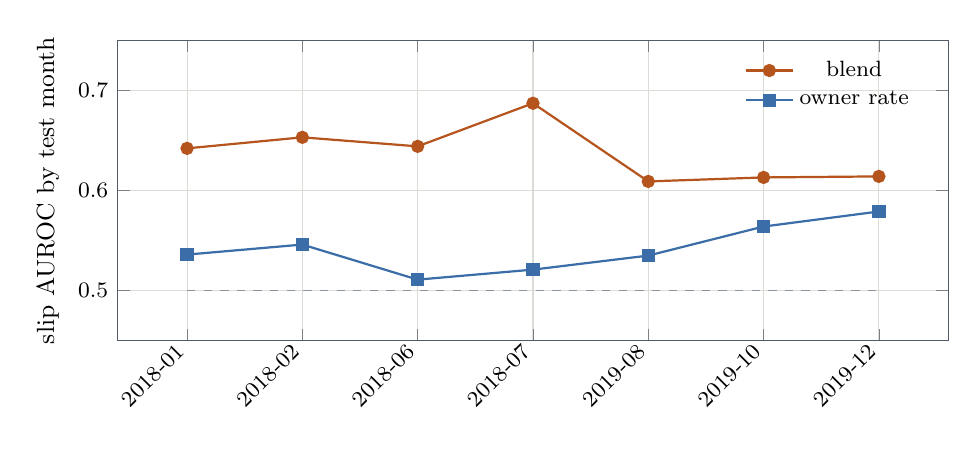
\begin{tikzpicture}
\begin{axis}[
  width=\textwidth, height=5.4cm, ymin=0.45, ymax=0.75,
  ylabel={slip AUROC by test month}, label style={font=\small}, tick label style={font=\footnotesize},
  symbolic x coords={2018-01,2018-02,2018-06,2018-07,2019-08,2019-10,2019-12}, xtick=data, x tick label style={rotate=45, anchor=east},
  grid=major, grid style={line}, axis line style={ink2},
  legend style={font=\footnotesize, at={(0.97,0.97)}, anchor=north east, draw=none, fill=none},
]
\addplot[copper, thick, mark=*] coordinates {(2018-01,0.642) (2018-02,0.653) (2018-06,0.644) (2018-07,0.687) (2019-08,0.609) (2019-10,0.613) (2019-12,0.614)};
\addplot[iso, thick, mark=square*] coordinates {(2018-01,0.536) (2018-02,0.546) (2018-06,0.511) (2018-07,0.521) (2019-08,0.535) (2019-10,0.564) (2019-12,0.579)};
\addplot[mute, dashed] coordinates {(2018-01,0.5) (2019-12,0.5)};
\legend{blend, owner rate}
\end{axis}
\end{tikzpicture}
\end{minipage}
\caption{Left: reliability of the blend's slip probabilities. Right: the honest model's edge over the owner-rate baseline is present in every test month and largest in 2018.}
\end{figure}

\subsection*{Reading the result}

\begin{itemize}
\item \textbf{Slip:} AUROC 0.62 and Brier 0.172 against 0.57 / 0.185 for the best simple baseline. Real, modest, and
  entirely carried by an upgrade's own public history: how long it has been listed, how often its date moved, its
  owner's track record. On upgrades never observed before, AUROC is 0.50.
\item \textbf{Cost:} no model beats a three-feature logistic regression, and none beats the base-rate Brier. Not material.
\item \textbf{Completion date:} PJM's own published date is a better point estimate (MAE 9.3 months) than any model's
  median (10.6). The useful model output is the interval: the survival P10--P90 band covers 78\% of outcomes at P90.
\item \textbf{Cancellation} is the strongest single signal in the data (AUROC 0.72).
\item \textbf{Why the classifier struggles:} a slip label is only decidable once its 12-month window has closed, so the
  labelled pool at any origin is older, shorter-horizon cohorts running a 4--7\% slip rate, while the 2018--2019 test
  months run 17--26\%, partly a real regime change. The survival formulation, which uses every observation with
  censoring, is the honest one for this label. At a 2018 origin the archive also offers at most about 28 months of
  follow-up, so multi-year completion quantiles are extrapolations and are flagged as such.
\end{itemize}

\section*{What both experiments say about the public record}

\begin{center}
\small
\begin{tabular}{p{0.3\textwidth}p{0.64\textwidth}}
\toprule
gap & effect \\
\midrule
Facility headroom (ratings, planning dispatch, contingency definitions) & In experiment 1 this, not topology, is what the public side cannot recover; better impedances buy three points. \\
Facility identity & Real PJM studies name facilities by PSS/E bus names; most public substations carry no name, so only a fifth of parsed findings could be placed. A bus-name dictionary would unlock the real-data benchmark. \\
Snapshot density and continuity & Experiment 2 has monthly snapshots in 2016--2017, quarterly later, none between December 2019 and September 2026, and only the baseline tab in the holdout years. \\
Label lag & A 12-month slip is only knowable a year after the promised date, which starves any classifier trained honestly on a short archive. \\
Milestones, permitting, procurement & Nothing public carries them; they are the obvious private inputs for a stronger upgrade model. \\
\bottomrule
\end{tabular}
\end{center}

Both prototypes are working point-in-time pipelines with leakage tests, chronological benchmarks, case studies and
small interfaces (a ranked-facility viewer for the first, a holdout browser and command-line scorer for the second).
Neither replaces an ISO study or a transmission owner's schedule, and neither should be read as an empirical claim beyond
what the tables above support. Questions I keep coming back to: whether ISO planning departments would recognise the
headroom-versus-topology split as the right way to describe the gap; whether there is a public or semi-public source of
bus-name-to-substation mappings I have missed; and whether anyone has seen the construction-status archive used this way
before.

\vspace{6pt}
{\small\color{ink2} Code, data manifests, reports and tests for both experiments are in the repository (\texttt{gridconstraint/} and \texttt{upgraderisk/}); every number here is copied from their generated reports.}

\end{document}
